\documentclass{beamer} 

\usepackage[utf8]{inputenc}
\usepackage[T1]{fontenc}       % Sinon Babel n'est pas content 
\usepackage{minted}            % Pour les blocs de code
\usepackage{amsfonts, amsmath} % Pour des symboles de maths
\usepackage{pgfplots}          % Pour les figures
\usepackage{mathtools}         % Des fractions dans des accolades
\usepackage[french]{babel}     % Pour le support de la langue française
\usepackage{hyperref}          % Pour des liens vers les références
\usepackage{subfigure} %pour afficher les graphes côte à côte
\usepackage{graphics}          % Pour les images

\useoutertheme{infolines} 

\definecolor{gold}{RGB}{254, 206, 0}

\setbeamercolor{title in head/foot}{bg=gold, fg=black}
\setbeamercolor{author in head/foot}{bg=myuniversity}
\setbeamertemplate{page number in head/foot}{}

\pgfplotsset{compat=1.18}

%\doublespacing{}

% Couleur des liens dans le document
\hypersetup{
  colorlinks = true,
  breaklinks,
  citecolor = [rgb]{.12,.54,.11},
  linkcolor = {blue},
  urlcolor = {blue},
}

\usetheme{Madrid}
\definecolor{myuniversity}{RGB}{0, 85, 150}
\usecolortheme[named=myuniversity]{structure}

\title[Lectures Dirigées]{Autour de la transformation de Fourier rapide}
%\subtitle{(Your Sub Title)}
%\institute[]{Rapport de lectures dirigées de L3 sous la supervision de Stéphane Balac}

\author[Samuel \& Ludovic]{Samuel Gallay et Ludovic Arnaud}

\institute[]{Rapport de lectures dirigées de L3\\
sous la supervision de Stéphane Balac}
\date{7 avril 2022}

\begin{document}

\begin{frame}
  \maketitle
\end{frame}

%\begin{frame}
%  \frametitle{Table des matières}
%  \tableofcontents
%\end{frame}

\section{Introduction}
\begin{frame}{Introduction}
   Objectif : évaluer numériquement une transformée de Fourier continue
   $$ \hat{f}(x) = \int_{-\infty}^{+\infty} f(t)e^{-itx}dt $$
   Quadrature de l'intégrale par la méthode des rectangles :
   \begin{equation*}
    \hat{f}(x) \approx \frac{a}{n}\sum_{j=0}^{n-1}f(t_j)e^{-i t_j x}
    \text{\ \ avec\ \ } t_j = -\frac{a}{2} + j \frac{a}{n}
  \end{equation*}
  
  \vspace{0.5cm}
    On suppose $f$ continue et à support dans $[-\frac{a}{2}, \frac{a}{2}]$.
   
\end{frame}

\begin{frame}{Calcul de $\hat{f}(x)$ en de nombreux points}
    Évaluation en un point : $O(n)$
    
    \vspace{0.3cm}
    Évaluation en $m$ points $(x_k)_{1 \le k \le m}$ : algorithme naïf en $O(n \times m)$

    \begin{center}
    \textcolor{orange}{Peut-on faire mieux ? Dans un cas particulier, oui !}
    \end{center}
    
    On suppose maintenant que $m$ = $n$ et que $x_k = -\frac{b}{2} + k \frac{b}{n}$
    
     \begin{exampleblock}{Algorithme classique}
        Par la transformation de Fourier rapide : $O(n\log{n})$
    \end{exampleblock}
    
    \begin{alertblock}{Contrainte}
        $$ab =2 \pi n$$
    \end{alertblock}
\end{frame}


\section{La transformation de Fourier discrète}
\begin{frame}{La transformation de Fourier discrète}

    \begin{block}{Définition de la transformation de Fourier discrète}
        $$D_k(z) = \sum_{j=0}^{n-1}z_j e^{-\frac{2i \pi j k}{n}} \text{\ \ et\ \ } D_k^{-1}(z) = \frac{1}{n}\sum_{j=0}^{n-1}z_j e^{\frac{2i \pi j k}{n}}$$
    \end{block}
    
    \begin{exampleblock}{Théorème d'inversion}
    $$z_k = D_k^{-1}\left( \left(D_j(z)\right)_{0\le j\le n-1} \right)$$
    \end{exampleblock}
    
    \begin{exampleblock}{Théorème de convolution circulaire}
        $$D_k(x*y) = D_k(x)\cdot D_k(y) \text{\ \ avec\ \ } (x*y)_l = \sum_{j=0}^{n-1}x_j y_{l-j}$$
    \end{exampleblock}
\end{frame}

\begin{frame}{Algorithme de Cooley-Tukey pour la FFT}
\begin{alertblock}{Attention !}
      Ne s'applique que dans le cas où $n$ est une puissance de $2$.
\end{alertblock}
    \begin{align*}
  D_k(z) &= D_k\left((z_{2j})_{0 \le j \le \frac{n}{2}-1}\right)
          +  e^{\frac{-2ik\pi}{n}}D_k\left((z_{2j+1})_{0 \le j \le \frac{n}{2}-1}\right) \\
  D_{\frac{n}{2} + k}(z) &= D_k\left((z_{2j})_{0 \le j \le \frac{n}{2}-1}\right)
          -  e^{\frac{-2ik\pi}{n}}D_k\left((z_{2j+1})_{0 \le j \le \frac{n}{2}-1}\right)
\end{align*}
    \begin{center}
    \textcolor{orange}{Approche de type \emph{diviser pour régner !}}
    \end{center}
    
\begin{exampleblock}{Calcul de sa complexité}
$$  C(n) = 2C\left(\frac{n}{2}\right) + \Theta(n) $$
Ainsi, $C(n) = \Theta(n\log(n))$ par le \emph{Master Theorem}.
\end{exampleblock}
\end{frame}

\begin{frame}{Retour au calcul des $\hat{f}(x_k)$}
    \begin{align*}
        \hat{f}(x_k) &\approx \frac{a}{n}\sum_{j=0}^{n-1}f(t_j)e^{-i t_j x_k}  
        =\frac{a}{n} \sum_{j=0}^{n-1}f(t_j)e^{-i (-\frac{a}{2}+j\frac{a}{n})(-\frac{b}{2}+k\frac{b}{n})} \\
        &=\frac{a}{n} \sum_{j=0}^{n-1}f(t_j)e^{-i\frac{ab}{4}}e^{i\frac{abk}{2n}}e^{i\frac{abj}{2n}}e^{-i\frac{abkj}{n^2}} \\
        &=\frac{a}{n} e^{-i\frac{ab}{4}}e^{i\frac{abk}{2n}}\sum_{j=0}^{n-1}f(t_j)e^{i\frac{abj}{2n}}e^{-i\frac{abkj}{n^2}} 
    \end{align*}
    \begin{center}
        \textcolor{orange}{On reconnaît une transformée de Fourier discrète ! \\ Mais avec une contrainte...}
    \end{center}
    \begin{alertblock}{Contrainte}
        $$ab =2 \pi n$$
    \end{alertblock}
\end{frame}

\begin{frame}{Impact de la contrainte}
\begin{center}
\begin{tikzpicture}
  \begin{axis}[
    xlabel={$t$}, ylabel={$u(t)$},
    title={Signal d'entrée ($n = 128$)}, 
    height=7cm, width=12cm, 
    grid=major]
    \addplot+[mark=+] table {gaussienne_entree.txt};
  \end{axis}
\end{tikzpicture}
\end{center}
\end{frame}

\begin{frame}{Impact de la contrainte}
\begin{tikzpicture}
  \begin{axis}[
    xlabel={$t$}, ylabel={$\hat{u}(t)$},
    title={Transformée de Fourier du signal}, 
    height=7cm, width=12cm, 
    grid=major]
    \addplot+[mark=+] table {gaussienne_sortie.txt};
  \end{axis}
\end{tikzpicture}
\end{frame}

\begin{frame}{Transformation de Fourier fractionnaire}
\begin{block}{Définition}
  $$G_k(x, \alpha)
  = \sum_{j=0}^{n-1}x_je^{-2i\pi jk\alpha} $$
\end{block}

Technique de Bluestein : $-2jk = - k^2 -j^2 + (k-j)^2 $. Ainsi :

$$G_k(x, \alpha) = e^{-i\pi \alpha k^2 } \sum_{j=0}^{n-1}x_je^{-i\pi\alpha j^2} e^{i\pi\alpha (k-j)^2}$$
\begin{center}
    \textcolor{orange}{C'est presque une convolution circulaire !}
\end{center}

\begin{exampleblock}{Complexité}
    Ainsi, $(G_k(x, \alpha))_{0\le k\le n-1}$ peut être calculé en $O(n\log(n))$ opérations par la FFT.
\end{exampleblock}
\end{frame}

\begin{frame}{Calcul des $\hat{f}(x_k)$ par la transformation fractionnaire}
    On reprend l'expression de $\hat{f}(x_k)$ précédente :
    \begin{align*}
        \hat{f}(x_k) &\approx \frac{a}{n} e^{-i\frac{ab}{4}}e^{i\frac{abk}{2n}}\sum_{j=0}^{n-1}f(t_j)e^{i\frac{ab}{2n}j}e^{-i\frac{ab}{n^2}jk} \\
         &\approx \frac{a}{n} e^{-i\frac{ab}{4}}e^{i\frac{abk}{2n}}\cdot G_k\left(\left( f(t_j)e^{i \frac{ab}{2n}j}\right)_{0 \le j < n},  \frac{ab}{2\pi n^2}\right) 
    \end{align*}
    \begin{center}
        \textcolor{orange}{On reconnaît une transformation de Fourier discrète fractionnaire !}
\end{center}
\begin{exampleblock}{Complexité}
  Ainsi, $(\hat{f}(x_k))_{0\le k\le n-1}$ peut être calculé en $O(n\log(n))$ opérations par la transformation fractionnaire rapide.
\end{exampleblock}
\end{frame}

\begin{frame}{Une nette amélioration}
\begin{tikzpicture}
  \begin{axis}[
    xlabel={$x$}, ylabel={$\hat{u}(x)$},
    title={Transformée de Fourier du signal}, 
    height=7cm, width=12cm, 
    grid=major]
    \addplot+[mark=+] table {gaussienne_sortie_bis.txt};
  \end{axis}
\end{tikzpicture}
\end{frame}

\begin{frame}{Inversion de Fourier}
  \begin{exampleblock}{Formule d'inversion de Fourier}
$$ f(t) = \frac{1}{2\pi}\int_{-\infty}^{+\infty} \hat{f}(x)e^{itx}dx $$
  \end{exampleblock}

En reprenant le raisonnement depuis le début on obtient :
\begin{align*}
f(t_j)  &\approx \frac{b}{2\pi n}\sum_{k=0}^{n-1}\hat{f}(x_k)e^{i x_k t_j} \\
      &\approx \frac{b}{2\pi n} e^{-i\frac{b}{2}t_j}\cdot G_j\left(\left( \hat{f}(x_k)e^{-i\frac{ab}{2n}k}\right)_{0 \le k < n},  -\frac{ab}{2\pi n^2}\right) 
\end{align*}
\begin{exampleblock}{Complexité}
  L'inverse aussi se calcule en $O(n\log(n))$ 
\end{exampleblock}
\end{frame}

\begin{frame}{Dérivation numérique via la FFT}
  \begin{exampleblock}{Dérivation et transformée de Fourier}
    Si de plus $f$ est continûment dérivable, $\hat{f'}(x)= ix\hat{f}(x)$   
  \end{exampleblock}
    \begin{center}
  \begin{tikzpicture}
    \begin{axis}[
      xlabel={$t$}, ylabel={$u'(t)$},
      title={Dérivée numérique de $u:t\mapsto e^{-\frac{t^2}{2}}$}, 
      height=5cm, width=10cm, 
      grid=major]
      \addplot+[mark=+] table {gaussienne_derivee.txt};
    \end{axis}
  \end{tikzpicture}
\end{center}

\end{frame}

\begin{frame}{L'équation de Schrödinger non-linéaire en optique}

  Voici le comportement d'une fibre optique :
\begin{equation*}
  \begin{dcases*}
    \frac{\partial u}{\partial z}(z, t) = - i\frac{\text{sign}(\beta_2)}{2} \frac{\partial^2 u}{{\partial t}^2}(z, t) + iN^2u(z, t)|u(z, t)|^2 \\
    u(0, t) = u_0(t)
  \end{dcases*}
\end{equation*}

\vspace{0.8cm}
Notons la ressemblance avec l'habituelle :
\begin{equation*}
  i\hbar \dot{\Psi} = \frac{-\hbar^2}{2m}\Delta\Psi + V\Psi
\end{equation*}
\end{frame}

\begin{frame}{La méthode \emph{split-step}}
  À la place de résoudre directement l'équation, on résout successivement les trois problèmes :
\begin{align*}
  \frac{\partial u_1}{\partial z}(z, t) &=   iN^2u_1(z, t)|u_1(z, t)|^2 
  & 
  u_1(0, t) = u(z_k, t) \\
  \frac{\partial u_2}{\partial z}(z, t) &= - i\frac{\text{sign}(\beta_2)}{2} \frac{\partial^2 u_2}{{\partial t}^2}(z, t)
  &
  u_2(z=0, t) = u_1(\frac{h}{2}, t) \\ 
  \frac{\partial u_3}{\partial z}(z, t) &=   iN^2u_3(z, t)|u_3(z, t)|^2
  &
  u_3(0, t) = u_2(h, t) 
\end{align*}

Et finalement : 
$u(z_{k+1}, t) = u(z_k + h, t) = u_3(\frac{h}{2}, t)$

\end{frame}


\begin{frame}{La méthode \emph{split-step}}
    On traite les deux parties non linéaires par une intégration, puis approximation de l'intégrale : 
    \begin{equation*}
      u_1(z, t) =  u(z_k, t)\cdot \text{exp}\left(\int_{0}^ziN^2|u_1(z, t)|^2dz\right)
    \end{equation*}

    Tandis que par une transformée de Fourier de $u_2$ par rapport à $t$, l'équation linéaire devient :
\begin{equation*}
  \frac{\partial \hat{u_2}}{\partial z}(z, \nu) = - i\frac{\text{sign}(\beta_2)}{2} (i\nu)^2\hat{u_2}(z, \nu) 
\end{equation*}

Le calcul explicite d'une solution est alors possible :
\begin{equation*}
  \hat{u_2}(h, \nu) 
= \hat{u_2}(z_k, \nu) \cdot e^{i\frac{\text{sign}(\beta_2)}{2} \nu^2 h} \label{eq_lin_solve}
\end{equation*}
\end{frame}
\section{Résultats et conclusion}

\begin{frame}{Résultats 1/3}
    Pour un signal d'entrée $u_0$ de la forme
    \begin{center}
  \begin{tikzpicture}
    \begin{axis}[
      ylabel={$|u_0(t)|^2$},
      height=4cm, width=10cm, 
      xmin=-3, xmax=3,
      grid=major]
      \addplot+[mark=+] table {FFT_u_entree.txt};
    \end{axis}
  \end{tikzpicture}
\end{center}
\begin{center}
  \begin{tikzpicture}
    \begin{axis}[ ylabel={$|\hat{u_0}(\nu)|^2$},
      height=4cm, width=10cm, 
      xmin=-3, xmax=3,
      grid=major]
      \addplot+[mark=+] table {FFT_uhat_entree.txt};
    \end{axis}
  \end{tikzpicture}
\end{center}
\end{frame}

\begin{frame}{Résultats 2/3}
    On obtient :
    \begin{center}
  \begin{tikzpicture}
    \begin{axis}[ ylabel={$|u(t)|^2$},
      height=4cm, width=10cm, 
      xmin=-3, xmax=3,
      grid=major]
      \addplot+[mark=+] table {FFT_u_sortie.txt};
    \end{axis}
  \end{tikzpicture}
\end{center}
\begin{center}
  \begin{tikzpicture}
    \begin{axis}[
    ylabel={$|\hat{u}(\nu)|^2$},
      height=4cm, width=10cm, 
      xmin=-3, xmax=3,
      grid=major]
      \addplot+[mark=+] table {FFT_uhat_sortie.txt};
    \end{axis}
  \end{tikzpicture}
\end{center}
\end{frame}

\begin{frame}{Résultats 3/3}
    La transformée de Fourier fractionnaire permet d'améliorer la précision. On prendra ici un facteur 2
    \begin{center}
  \begin{tikzpicture}
    \begin{axis}[
      ylabel={$|u(t)|^2$},
      height=4cm, width=10cm, 
      xmin=-3, xmax=3,
      grid=major]
      \addplot+[mark=+] table {FrFFT_u_sortie.txt};
    \end{axis}
  \end{tikzpicture}
\end{center}
\begin{center}
  \begin{tikzpicture}
    \begin{axis}[
      ylabel={$|\hat{u}(\nu)|^2$},
      height=4cm, width=10cm, 
      xmin=-3, xmax=3,
      grid=major]
      \addplot+[mark=+] table {FrFFT_uhat_sortie.txt};
    \end{axis}
  \end{tikzpicture}
\end{center}
\end{frame}



\begin{frame}
  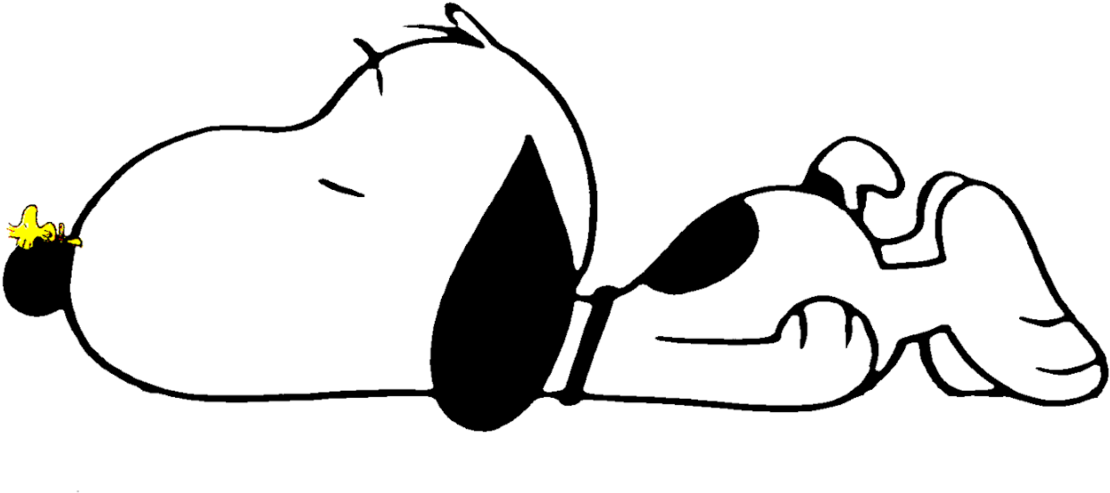
\includegraphics[scale=0.3]{snoopy}
  \begin{center}
    \textcolor{purple}{\huge Merci pour votre attention !}
  \end{center}
\end{frame}

\begin{frame}{Bibliographie}
\nocite{FOURINT}
\nocite{FRAC}
\bibliographystyle{plainnat-fr}
\bibliography{biblio}
\end{frame}

\end{document}
